\documentclass[10pt,letterpaper]{article}
%\usepackage{toolsper}
\usepackage{amsmath,geometry,amssymb,xepersian}
\newcommand{\eqn}[1]{
\begin{equation}
\begin{split}
#1
%\label{#2}
\end{split}
\end{equation}
}
%%%%%%%%%%%%%

%       \eqn{
%       x=x^2
%       }{label}

%%%%%%%%%%%%%
\newcommand{\feqn}[2]{
\begin{tcolorbox}[width=7in, colback=white]
\begin{equation}
\begin{split}
#1
\label{#2}
\end{split}
\end{equation}
\end{tcolorbox}
}
%%%%%%%%%%%%%%%
\newcommand{\hl}{
\begin{center}
\line(1,0){450}
\end{center}}
%%%%%%%%%%%%%%%
\newcommand{\qn}[2]{
\[
\begin{split}
#1
\label{#2}
\end{split}
\]
}
%\settextfont{B Nazanin}
\usepackage{lipsum}
\setlength{\parindent}{0mm}
\setlength{\parskip}{3mm}
\newcommand{\pic}[2]{
\begin{center}
\includegraphics[width=#2]{#1}
\end{center}
}
\begin{document}
\Large
\begin{center}
به نام او

پاسخ تمرینات سری یازدهم درس احتمال مهندسی

\hrulefill
\end{center}
سوال 1)

بنا به تعریف و خواص چگالی های احتمال:
\eqn{
&f_X(x)=\int_{-\infty}^\infty f_{XY}(x,y)dy
\\&E\{X\}=\int_{-\infty}^\infty xf_{X}(x)dx=\int_{-\infty}^\infty xf_{XY}(x,y)dxdy
\\&E\{XY\}=\int_{-\infty}^\infty xyf_{XY}(x,y)dxdy
}

الف) 
\eqn{
f_X(x)&=\int \frac{1}{\pi}e^{-x^2-y^2}dy
\\&=\int \frac{1}{\pi}e^{-x^2}e^{-y^2}dy
\\&=\frac{1}{\pi}e^{-x^2}\int e^{-y^2}dy
\\&=\frac{1}{\sqrt\pi}e^{-x^2}{1\over \sqrt \pi}\int e^{-y^2}dy
\\&=\frac{1}{\sqrt\pi}e^{-x^2}
}

\eqn{
E\{X\}=\int \frac{x}{\sqrt\pi}e^{-x^2} dx=0
}
زیرا $\frac{1}{\sqrt\pi}e^{-x^2}$ یک تابع فرد روی اعداد حقیقی است.

\eqn{
E\{XY\}&=\iint xy\frac{1}{\pi}e^{-x^2-y^2}dxdy
\\&=\iint xy\frac{1}{\pi}e^{-x^2}e^{-y^2}dxdy
\\&=\frac{1}{\pi}\int xe^{-x^2}dx\int ye^{-y^2}dy=0
}

ب) 
\eqn{
f_X(x)&=\int_{|x-1|+|y-1|<1} {3\over 2}(1-|x-1|-|y-1|)dy
}
با تغییر متغیر 
$
y\to y+1
$
می توان نوشت:
\eqn{
f_X(x)&=\int_{|x-1|+|y|<1} {3\over 2}(1-|x-1|-|y|)dy
}
از آنجا که ناحیه 
$
|x-1|+|y|<1
$
و تابع 
$
{3\over 2}(1-|x-1|-|y|)
$
هر دو نسبت به $y$ زوج هستند، می توان انتگرال را تنها برای 
$
y>0
$
حساب نموده و مقدار آن را دو برابر کرد؛ به عبارت دیگر:
\eqn{
f_X(x)&=2\int_{|x-1|+|y|<1,y>0} {3\over 2}(1-|x-1|-y)dy
\\&=3\int_{y=0}^{1-|x-1|} 1-|x-1|-ydy
\\&=3(1-|x-1|)y-3{y^2\over 2}\Big|_{y=0}^{1-|x-1|}
\\&={3\over 2}(1-|x-1|)^2\quad,\quad 0<x<2
}
بنابراین 
$$
f_X(x)=\begin{cases}
{3\over 2}(1-|x-1|)^2&,\quad 0<x<2\\
0&,\quad \text{سایر جاها}
\end{cases}
$$
دو روش برای محاسبه امید ریاضی $X$ وجود دارد. روش اول، روش مستقیم انتگرال گیری است. روش دوم این است که توجه کنیم که چگالی احتمال $X$ حول $x=1$ متقارن است. به سادگی می توان گفت که امید ریاضی $X$ باید برابر 1 باشد.

\eqn{
E\{XY\}&=\int_{|x-1|+|y-1|<1} xy{3\over 2}(1-|x-1|-|y-1|)dxdy
\\&=\int_{|u|+|w|<1} (u+1)(w+1){3\over 2}(1-|u|-|w|)dudw
\\&=\int_{|u|+|w|<1} uw{3\over 2}(1-|u|-|w|)dudw
\\&+\int_{|u|+|w|<1} u{3\over 2}(1-|u|-|w|)dudw
\\&+\int_{|u|+|w|<1} w{3\over 2}(1-|u|-|w|)dudw
\\&+\int_{|u|+|w|<1} {3\over 2}(1-|u|-|w|)dudw
}
از 4 انتگرال آخر، سه انتگرال اول برابر صفرند زیرا تابع تحت انتگرال نسبت به $u$ و $w$ فرد بوده و بازه انتگرال گیری نیز متقارن است. در این صورت:
\eqn{
E\{XY\}&=\int_{|u|+|w|<1} {3\over 2}(1-|u|-|w|)dudw
\\&=4\int_{|u|+|w|<1,u>0,w>0} {3\over 2}(1-|u|-|w|)dudw
\\&=6\int_{u+w<1,u>0,w>0} (1-u-w)dudw
\\&=6\int_0^1\int_0^{1-w} (1-u-w)dudw
\\&=6\int_0^1 (1-w)u-{u^2\over 2}\Big|_0^{1-w}dw
\\&=3\int_0^1 (1-w)^2dw=1
}

پ)
\eqn{
f_X(x)&=\int_x^1e^{1-x}dy=(1-x)e^{1-x}
}
بنابراین
$$
f_{X}(x)=\begin{cases}
(1-x)e^{1-x}&,\quad 0<x<1\\
0&,\quad \text{سایر جاها}
\end{cases}
$$
برای محاسبه امید ریاضی:
\eqn{
E\{X\}&=\int_0^1 x(1-x)e^{1-x}dx
\\&=\int_0^1 u(1-u)e^{u}du
\\&=\int_0^1 (u-u^2)e^{u}du
}
برای محاسبه انتگرال فوق به روش جزء به جزء، ابتدا مشتقات متوالی $u-u^2$ و سپس انتگرال های متوالی $e^u$ را محاسبه کرده و با علامت های مثبت و منفی متناوبا در هم ضرب می کنیم؛ به عبارت دیگر:
\begin{figure}[htbp]
\centering
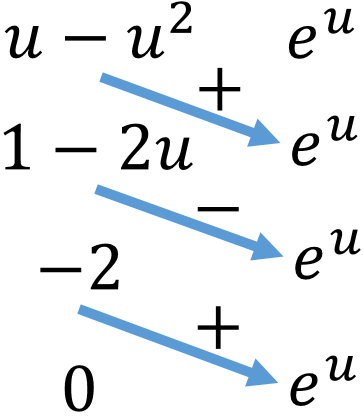
\includegraphics[width=30mm]{ibp_hw11.png}
\end{figure}
بنابراین
\eqn{
E\{X\}&=\int_0^1 (u-u^2)e^{u}du
\\&=(u-u^2)e^{u}-(1-2u)e^{u}+(-2)e^u\Big|_0^1=3-e
}
همچنین
\eqn{
E\{XY\}&=\int_0^1\int_x^1 xye^{1-x}dydx
\\&=\int_0^1 x(1-{x^2\over 2})e^{1-x}dx=6-2e
}

ت) X و Y، دو متغیر تصادفی گسسته (با مقادیر صحیح) اند و pmf آنها به صورت زیر است:
$
p_{X,Y}(x,y)=\begin{cases}
\frac{1}{16}&,\quad x^2+y^2\le 10 \ \ ,\ \ x\ge y\\
0&,\quad \text{سایر جاها}
\end{cases}
$
(در صورت سوال، مقدار $1\over 16$ باید به $1\over 21$ تغییر پیدا کند!)

جدول pmf به صورت زیر است ($p=21$):
\begin{figure}[htbp]
\centering
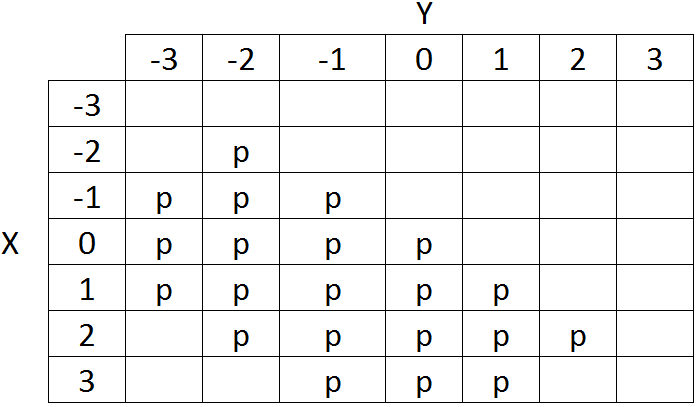
\includegraphics[width=80mm]{hw11_pmf.png}
\end{figure}

در این صورت:
\eqn{
&\Pr\{X=x\}=\begin{cases}
{1\over 21}&,\quad x=-2\\
{1\over 7}&,\quad x=-1\\
{4\over 21}&,\quad x=0\\
{5\over 21}&,\quad x=1\\
{5\over 21}&,\quad x=2\\
{1\over 7}&,\quad x=3\\
\end{cases}
}

همچنین
\eqn{
E\{X\}=\sum_x x\cdot\Pr\{X=x\}={13\over 21}
}

\eqn{
E\{XY\}=\sum_{x,y} xy\Pr\{X=x,Y=y\}={5\over21}
}

سوال 2) الف) به وضوح 
\eqn{
&\mu_X=E\{X\}=p_3+p_4
\\&\mu_Y=E\{Y\}=p_2+p_4
}{}
در نتیجه
\eqn{
&\text{\lr{cov}}(X,Y)=E\{(X-\mu_X)(Y-\mu_Y)\}
\\&=E\{XY\}-\mu_X\mu_Y
\\&=p_4-(p_2+p_4)(p_3+p_4)
}{}
در نتیجه برای صفر بودن کوواریانس باید داشته باشیم 
$
p_4=(p_2+p_4)(p_3+p_4)
$
.

ب) شرط همبستگی که در قسمت قبلی به دست آمد. برای استقلال باید داشته باشیم:
\eqn{
&p_1=(p_1+p_3)(p_1+p_2)
\\&p_2=(p_1+p_2)(p_2+p_4)
\\&p_3=(p_1+p_3)(p_3+p_4)
\\&p_4=(p_2+p_4)(p_3+p_4)
}{}
%از جمع هر چهار معادله‌ی فوق نتیجه می شود:
%\eqn{
%&p_1+p_2+p_3+p_4=
%p_1^2+p_2^2+p_3^2+p_4^2
%\\&+2p_1p_2+2p_1p_3+2p_1p_4
%\\&+2p_2p_3+2p_2p_4+2p_3p_4
%\\&\implies 1=1
%}{}
%بنابراین این 4 معادله از هم مستقل نیستند و می توان هر یک از این 4 معادله را حذف کرد. با حذف معادله‌ی 1، به معادلات زیر می رسیم:
%\eqn{
%&p_2=(1-p_3-p_4)(p_2+p_4)
%\\&p_3=(1-p_2-p_4)(p_3+p_4)
%\\&p_4=(p_2+p_4)(p_3+p_4)
%}{}
%از دو معادله‌ی اوب 
نکته اینجاست که
\begin{enumerate}
\item
از معادله‌ی 4، با کم کردن 
$
p_2+p_4
$
 به معادله‌ی 2 می رسیم.
\item
از معادله‌ی 4، با کم کردن 
$
p_3+p_4
$
 به معادله‌ی 3 می رسیم.
\item
از جمع معادله‌های 2، 3 و 4 به معادله‌ی 1 می رسیم.
\end{enumerate}
بنابراین در این سوال، 
\textbf{
ناهمبستگی و استقلال معادلند.
}
\newline\newline
سوال 3) الف) به سادگی و با انتگرال گیری می توان نتیجه گرفت:
\eqn{
&f_X(x)=\begin{cases}
1&,\quad 0<x<1
\\0&,\quad \text{در غیر این صورت}
\end{cases}
\\&f_Y(y)=\begin{cases}
1&,\quad 0<y<1
\\0&,\quad \text{در غیر این صورت}
\end{cases}
}{}
در نتیجه
\eqn{
E\{X\}=E\{Y\}={1\over 2}
}{}
هم چنین می دانیم
\eqn{
E\{XY\}&=\int_0^1\int_0^1 xy+\alpha xy\sin[2\pi(x+y)]dxdy
\\&={1\over 4}+\alpha\int_0^1\int_0^1 xy\sin[2\pi(x+y)]dxdy
\\&={1\over 4}+\alpha\int_0^1y\int_0^1 x\sin[2\pi(x+y)]dxdy
}{}
هم چنین
\eqn{
\int_0^1 x\sin[2\pi(x+y)]dx&=\left[-{x\over 2\pi}\cos[2\pi(x+y)]+{1\over 4\pi^2}\sin[2\pi(x+y)]\right]_{x=0}^{x=1}
\\&=-{\cos 2\pi y\over 2\pi}
}{}
در نتیجه
\eqn{
E\{XY\}&=
{1\over 4}-{\alpha\over 2\pi}\int_0^1y{\cos 2\pi y}dy
\\&={1\over 4}-{\alpha\over 2\pi}\left[{y\sin 2\pi y\over 2\pi}+{\cos 2\pi y\over 4\pi^2}\right]_{y=0}^{y=1}
\\&={1\over 4}
}{}
از آنجا که همواره 
$
E\{XY\}=E\{X\}E\{Y\}
$
، در نتیجه همواره دو متغیر تصادفی $X$ و $Y$ ناهمبسته هستند.

ب) به سادگی دیده می شود که 
$$
f_{X,Y}(x,y)=f_X(x)f_Y(y)\iff \alpha=0
$$

سوال 4) الف) با توجه به اینکه 
$
\Pr\{XY>1\}=0
$
 ، برای $u<1$ خواهیم داشت:
\qn{
&\Pr\{XY<u\}=\Pr\left\{X<{u\over Y}\right\}
\\&=\int_{-\infty}^\infty \Pr\left\{X<{u\over y}|Y=y\right\}f_Y(y)dy
\\&=\int_0^1 \Pr\left\{X<{u\over y}|Y=y\right\}dy
\\&=\int_0^u \Pr\left\{X<{u\over y}\right\}dy
\\&+
\int_u^1 \Pr\left\{X<{u\over y}\right\}dy
\\&=u+\int_u^1 {u\over y}dy
\\&=u-u\ln u
}{}
بنابراین
\qn{
f_{XY}(u)={d\over du}F_{XY}(u)=
\begin{cases}
-\ln u&,\quad 0\le u<1
\\0&,\quad \text{\rl{در غیر این صورت}}
\end{cases}
}{}
ب) ابتدا، می دانیم
\qn{
\Pr\{X+Y<0\}=1-\Pr\{X+Y<2\}=0
}{}
بنابراین با فرض 
$
0<u<2
$
 خواهیم داشت:
\qn{
&\Pr\{X+Y<u\}=\Pr\left\{X<{u-Y}\right\}
\\&=\int_{-\infty}^\infty \Pr\left\{X<{u-y}|Y=y\right\}f_Y(y)dy
\\&=\int_0^1 \Pr\left\{X<{u-y}|Y=y\right\}dy
%\\&=\int_0^u \Pr\left\{X<{u-y}\right\}dy
%\\&+
%\int_u^1 \Pr\left\{X<{u\over y}\right\}dy
%\\&=u+\int_u^1 {u\over y}dy
%\\&=u-u\ln u
}{}
به ازای $u<1$:
\qn{
&\int_0^1 \Pr\left\{X<{u-y}|Y=y\right\}dy\\&=\int_0^u \Pr\left\{X<{u-y}|Y=y\right\}dy
\\&=\int_0^u u-ydy\\&={u^2\over 2}
}{}
به ازای $u>1$:
\qn{
&\int_0^1 \Pr\left\{X<{u-y}|Y=y\right\}dy\\&=\int_{u-1}^1 \Pr\left\{X<{u-y}|Y=y\right\}dy
\\&+
\int_0^{u-1} \Pr\left\{X<{u-y}|Y=y\right\}dy
\\&=\int_{u-1}^1 u-ydy\\&+u-1
\\&=u(2-u)-{1\over 2}+{(u-1)^2\over 2}+u-1
\\&=2u-{u^2\over 2}
}{}
بنابراین
\qn{
f(x)=
\begin{cases}
x&,\quad 0<x<1
\\2-x&,\quad 1\le x<2
\\0&,\quad\text{\rl{در غیر این صورت}}
\end{cases}
}{}
پ) به ازای $u>0$
\qn{
&\Pr\left\{{X\over Y}<u\right\}=\Pr\left\{X<uY\right\}
\\&=\int_{-\infty}^\infty \Pr\left\{X<uy|Y=y\right\}f_Y(y)dy
\\&=\int_0^1 \Pr\left\{X<uy|Y=y\right\}dy
%\\&=\int_0^u \Pr\left\{X<{u-y}\right\}dy
%\\&+
%\int_u^1 \Pr\left\{X<{u\over y}\right\}dy
%\\&=u+\int_u^1 {u\over y}dy
%\\&=u-u\ln u
}{}
به ازای $u<1$ با اندکی محاسبات
\qn{
\Pr\left\{{X\over Y}<u\right\}={u\over 2}
}{}
به ازای $u>1$ با اندکی محاسبات بیشتر
\qn{
\Pr\left\{{X\over Y}<u\right\}=1-{1\over 2u}
}{}
بنابراین
\qn{
f(x)=
\begin{cases}
{1\over 2}&,\quad 0<x<1
\\{1\over 2x^2}&,\quad 1\le x
\\0&,\quad\text{\rl{در غیر این صورت}}
\end{cases}
}{}
ت) با فرض 
$
0<u<1
$
 خواهیم داشت:
\qn{
&\Pr\left\{\max\{X,Y\}<u\right\}=\Pr\left\{X<u,Y<u\right\}
\\&=\Pr\left\{X<u\right\}\Pr\left\{Y<u\right\}
=u^2
}{}
بنابراین
\qn{
f(x)=
\begin{cases}
2x&,\quad 0<x<1
\\0&,\quad\text{\rl{در غیر این صورت}}
\end{cases}
}{}
ث) با فرض 
$
0<u<1
$
 خواهیم داشت:
\qn{
&\Pr\left\{\min\{X,Y\}<u\right\}=1-\Pr\left\{\min\{X,Y\}>u\right\}
\\&=1-\Pr\left\{X>u,Y>u\right\}
\\&=1-\Pr\left\{X>u\right\}\Pr\left\{Y>u\right\}
=1-(1-u)^2
}{}
بنابراین
\qn{
f(x)=
\begin{cases}
2-2x&,\quad 0<x<1
\\0&,\quad\text{\rl{در غیر این صورت}}
\end{cases}
}{}
اکنون اگر متغیرهای تصادفی $X$ و $Y$، نمایی با پارامتر 1 باشند، در این صورت با فرض 
$
u>0
$

ب)
\qn{
&\Pr\left\{X+Y<u\right\}=\Pr\left\{X<u-Y\right\}
\\&=\int_0^\infty e^{-y}\Pr\left\{X<u-y\right\}dy
\\&=\int_0^u e^{-y}\Pr\left\{X<u-y\right\}dy
\\&=\int_0^u e^{-y}(1-e^{y-u})dy
\\&=\int_0^u e^{-y}-e^{-u}dy
\\&=1-e^{-u}-ue^{-u}
}{}
در نتیجه
\qn{
f(x)=xe^{-x}\quad,\quad x>0
}{}
پ)
\qn{
&\Pr\left\{{X\over Y}<u\right\}=\Pr\left\{X<uY\right\}
\\&=\int_0^\infty e^{-y}\Pr\left\{X<uy\right\}dy
%\\&=\int_0^u e^{-y}\Pr\left\{X<u-y\right\}dy
\\&=\int_0^\infty e^{-y}(1-e^{-yu})dy
\\&=\int_0^\infty e^{-y}-e^{-(1+u)y}dy
\\&=1-{1\over u+1}
}{}
در نتیجه
\qn{
f(u)={1\over (u+1)^2}
\quad,\quad u>0
}{}
%
%چ) $X+Y$
%
%ح) $X\over Y$
\end{document}